\documentclass{ximera}
\graphicspath{  %% When looking for images,
{./}            %% look here first,
{./pictures/}   %% then look for a pictures folder,
{../pictures/}  %% which may be a directory up.
{../../pictures/}  %% which may be a directory up.
{../../../pictures/}  %% which may be a directory up.
{../../../../pictures/}  %% which may be a directory up.
}

\usepackage{listings}
%\usepackage{circuitikz}
\usepackage{xcolor}
\usepackage{amsmath,amsthm}
\usepackage{subcaption}
\usepackage{graphicx}
\usepackage{tikz}
%\usepackage{tikz-3dplot}
\usepackage{amsfonts}
%\usepackage{mdframed} % For framing content
%\usepackage{tikz-cd}

  \renewcommand{\vector}[1]{\left\langle #1\right\rangle}
  \newcommand{\arrowvec}[1]{{\overset{\rightharpoonup}{#1}}}
  \newcommand{\ro}{\texttt{R}}%% row operation
  \newcommand{\dotp}{\bullet}%% dot product
  \renewcommand{\l}{\ell}
  \let\defaultAnswerFormat\answerFormatBoxed
  \usetikzlibrary{calc,bending}
  \tikzset{>=stealth}
  




%make a maroon color
\definecolor{maroon}{RGB}{128,0,0}
%make a dark blue color
\definecolor{darkblue}{RGB}{0,0,139}
%define the color fourier0 to be the maroon color
\definecolor{fourier0}{RGB}{128,0,0}
%define the color fourier1 to be the dark blue color
\definecolor{fourier1}{RGB}{0,0,139}
%define the color fourier 1t to be the light blue color
\definecolor{fourier1t}{RGB}{173,216,230}
%define the color fourier2 to be the dark green color
\definecolor{fourier2}{RGB}{0,100,0}
%define teh color fourier2t to be the light green color
\definecolor{fourier2t}{RGB}{144,238,144}
%define the color fourier3 to be the dark purple color
\definecolor{fourier3}{RGB}{128,0,128}
%define the color fourier3t to be the light purple color
\definecolor{fourier3t}{RGB}{221,160,221}
%define the color fourier0t to be the red color
\definecolor{fourier0t}{RGB}{255,0,0}
%define the color fourier4 to be the orange color
\definecolor{fourier4}{RGB}{255,165,0}
%define the color fourier4t to be the darker orange color
\definecolor{fourier4t}{RGB}{255,215,0}
%define the color fourier5 to be the yellow color
\definecolor{fourier5}{RGB}{255,255,0}
%define the color fourier5t to be the darker yellow color
\definecolor{fourier5t}{RGB}{255,255,100}
%define the color fourier6 to be the green color
\definecolor{fourier6}{RGB}{0,128,0}
%define the color fourier6t to be the darker green color
\definecolor{fourier6t}{RGB}{0,255,0}

%New commands for this doc for errors in copying
\newcommand{\eigenvar}{\lambda}
%\newcommand{\vect}[1]{\mathbf{#1}}
\renewcommand{\th}{^{\text{th}}}
\newcommand{\st}{^{\text{st}}}
\newcommand{\nd}{^{\text{nd}}}
\newcommand{\rd}{^{\text{rd}}}
\newcommand{\paren}[1]{\left(#1\right)}
\newcommand{\abs}[1]{\left|#1\right|}
\newcommand{\R}{\mathbb{R}}
\newcommand{\C}{\mathbb{C}}
\newcommand{\Hilb}{\mathbb{H}}
\newcommand{\qq}[1]{\text{#1}}
\newcommand{\Z}{\mathbb{Z}}
\newcommand{\N}{\mathbb{N}}
\newcommand{\q}[1]{\text{``#1''}}
%\newcommand{\mat}[1]{\begin{bmatrix}#1\end{bmatrix}}
\newcommand{\rref}{\text{reduced row echelon form}}
\newcommand{\ef}{\text{echelon form}}
\newcommand{\ohm}{\Omega}
\newcommand{\volt}{\text{V}}
\newcommand{\amp}{\text{A}}
\newcommand{\Seq}{\textbf{Seq}}
\newcommand{\Poly}{\textbf{P}}
\renewcommand{\quad}{\text{    }}
\newcommand{\roweq}{\simeq}
\newcommand{\rowop}{\simeq}
\newcommand{\rowswap}{\leftrightarrow}
\newcommand{\Mat}{\textbf{M}}
\newcommand{\Func}{\textbf{Func}}
\newcommand{\Hw}{\textbf{Hamming weight}}
\newcommand{\Hd}{\textbf{Hamming distance}}
\newcommand{\rank}{\text{rank}}
\newcommand{\longvect}[1]{\overrightarrow{#1}}
% Define the circled command
\newcommand{\circled}[1]{%
  \tikz[baseline=(char.base)]{
    \node[shape=circle,draw,inner sep=2pt,red,fill=red!20,text=black] (char) {#1};}%
}

% Define custom command \strikeh that just puts red text on the 2nd argument
\newcommand{\strikeh}[2]{\textcolor{red}{#2}}

% Define custom command \strikev that just puts red text on the 2nd argument
\newcommand{\strikev}[2]{\textcolor{red}{#2}}

%more new commands for this doc for errors in copying
\newcommand{\SI}{\text{SI}}
\newcommand{\kg}{\text{kg}}
\newcommand{\m}{\text{m}}
\newcommand{\s}{\text{s}}
\newcommand{\norm}[1]{\left\|#1\right\|}
\newcommand{\col}{\text{col}}
\newcommand{\sspan}{\text{span}}
\newcommand{\proj}{\text{proj}}
\newcommand{\set}[1]{\left\{#1\right\}}
\newcommand{\degC}{^\circ\text{C}}
\newcommand{\centroid}[1]{\overline{#1}}
\newcommand{\dotprod}{\boldsymbol{\cdot}}
%\newcommand{\coord}[1]{\begin{bmatrix}#1\end{bmatrix}}
\newcommand{\iprod}[1]{\langle #1 \rangle}
\newcommand{\adjoint}{^{*}}
\newcommand{\conjugate}[1]{\overline{#1}}
\newcommand{\eigenvarA}{\lambda}
\newcommand{\eigenvarB}{\mu}
\newcommand{\orth}{\perp}
\newcommand{\bigbracket}[1]{\left[#1\right]}
\newcommand{\textiff}{\text{ if and only if }}
\newcommand{\adj}{\text{adj}}
\newcommand{\ijth}{\emph{ij}^\text{th}}
\newcommand{\minor}[2]{M_{#2}}
\newcommand{\cofactor}{\text{C}}
\newcommand{\shift}{\textbf{shift}}
\newcommand{\startmat}[1]{
  \left[\begin{array}{#1}
}
\newcommand{\stopmat}{\end{array}\right]}
%a command to give a name to explorations and hints and theorems
\newcommand{\name}[1]{\begin{centering}\textbf{#1}\end{centering}}
\newcommand{\vect}[1]{\vec{#1}}
\newcommand{\dfn}[1]{\textbf{#1}}
\newcommand{\transpose}{\mathsf{T}}
\newcommand{\mtlb}[2][black]{\texttt{\textcolor{#1}{#2}}}
\newcommand{\RR}{\mathbb{R}} % Real numbers
\newcommand{\id}{\text{id}}
\newcommand{\coord}[1]{\langle#1\rangle}
\newcommand{\RREF}{\text{RREF}}
\newcommand{\Null}{\text{Null}}
\newcommand{\Nullity}{\text{Nullity}}
\newcommand{\Rank}{\text{Rank}}
\newcommand{\Col}{\text{Col}}
\newcommand{\Ef}{\text{EF}}
\newcommand{\boxprod}[3]{\abs{(#1\times#2)\cdot#3}}

\author{Zack Reed}

\title{Images and Kernels of Transformations}

\begin{document}
\begin{abstract}

\end{abstract}
\maketitle

\section*{Image and Kernel of a Linear Transformation}

In a previous activity we observed that the image of the linear transformation $T$ is the same as the span of the columns of the associated matrix $A$. We also saw that we could exactly describe the images of linear transformations, as well as their kernels (aka the null space of the associated matrix).
 
\subsection*{Nullity and the Kernel of a Linear Transformation}
 
Before, we discussed how the \emph{kernel} of a linear transformation is all vectors that map to $\vec{0}$, that is, $\vec{v}$ such that $T(\vec{v})=\vec{0}$. For the sake of again using different verbiage for the same thing, it is worth stating that the kernel of a transformation is the null space of its matrix.



$$\mbox{ker}(T)=\mbox{null}(A).$$
 
\begin{example}\label{ex:kernel} Let $T:\RR^5\rightarrow \RR^4$ be a linear transformation with standard matrix $$A=\begin{bmatrix}1 & 2 & 2 &-1 & 0\\-1 & 3 & 1 & 0 & -1\\3 & 0 & 0 & 3 & 6\\ 1 & -1 & 1 & -2 & -1\end{bmatrix}$$
\begin{enumerate}
\item \label{item:kernelT}
Find $\mbox{ker}(T)$
\item \label{item:dimkernelT}
Find $\mbox{dim}(\mbox{ker}(T))$.
\end{enumerate}
\begin{explanation}

\ref{item:kernelT} We did this before, in the previous section, however it's always good to practice. To find the kernel of $T$, we need to find all vectors of $\RR^5$ that map to $\vec{0}$ in $\RR^4$.  This amounts to solving the equation $A\vec{x}=\vec{0}$.
 
\texttt{rref(A)} yields:
 
$$\mbox{rref}(A)= \begin{bmatrix} 1 & 0 & 0 & 1 & 2\\0 & 1 & 0 & 1 & 1\\0 & 0 & 1 & -2 & -2\\ 0 & 0 & 0 & 0 & 0 \end{bmatrix}$$
 
From our work with null spaces, we can form vectors whose linear combinations form the kernel of $T$:
$$\mbox{ker}(T)=\begin{bmatrix}\answer{-1}\\-1\\\answer{2}\\\answer{1}\\0\end{bmatrix}s+\begin{bmatrix}\answer{-2}\\-1\\2\\0\\\answer{1}\end{bmatrix}t$$
 
\end{explanation}
\end{example}
 
Recall that the \dfn{null space} of a matrix $A$ is defined to be set of all solutions to the homogeneous equation $A\vec{x}=\vec{0}$. This means that  if $T:\RR^n\rightarrow \RR^m$ is a linear transformation with standard matrix $A$ then
$$\mbox{ker}(T)=\mbox{null}(A)$$
 
START ACTUAL Here


\section*{Image and Kernel of a Linear Transformation}

We're now going to focus again on properties of linear transformations, which will then help us determine criteria for invertibility of matrices.

\subsection*{The Image of a Linear Transformation}

A few times throughout the course so far, we've encountered a phenomenon in which matrices ``squish'' space down to a smaller dimension. For instance, if we take the point cloud from $\texttt{mug.mat}$ as a representation of unaltered space and apply the matrix $A=\begin{bmatrix}
  1&0&1\\0&2&2\\1&2&3
\end{bmatrix}$, we see that the result of multiplication by $A$ squishes the mug down to the diagonal plane shown below. 

\begin{verbatim}
  A=[1 0 1;
  0 2 2;
  1 2 3]
  linalg.plot_cloud_with_vectors(mug);
  linalg.plot_cloud_with_vectors(A*mug);
\end{verbatim}



\begin{center}
  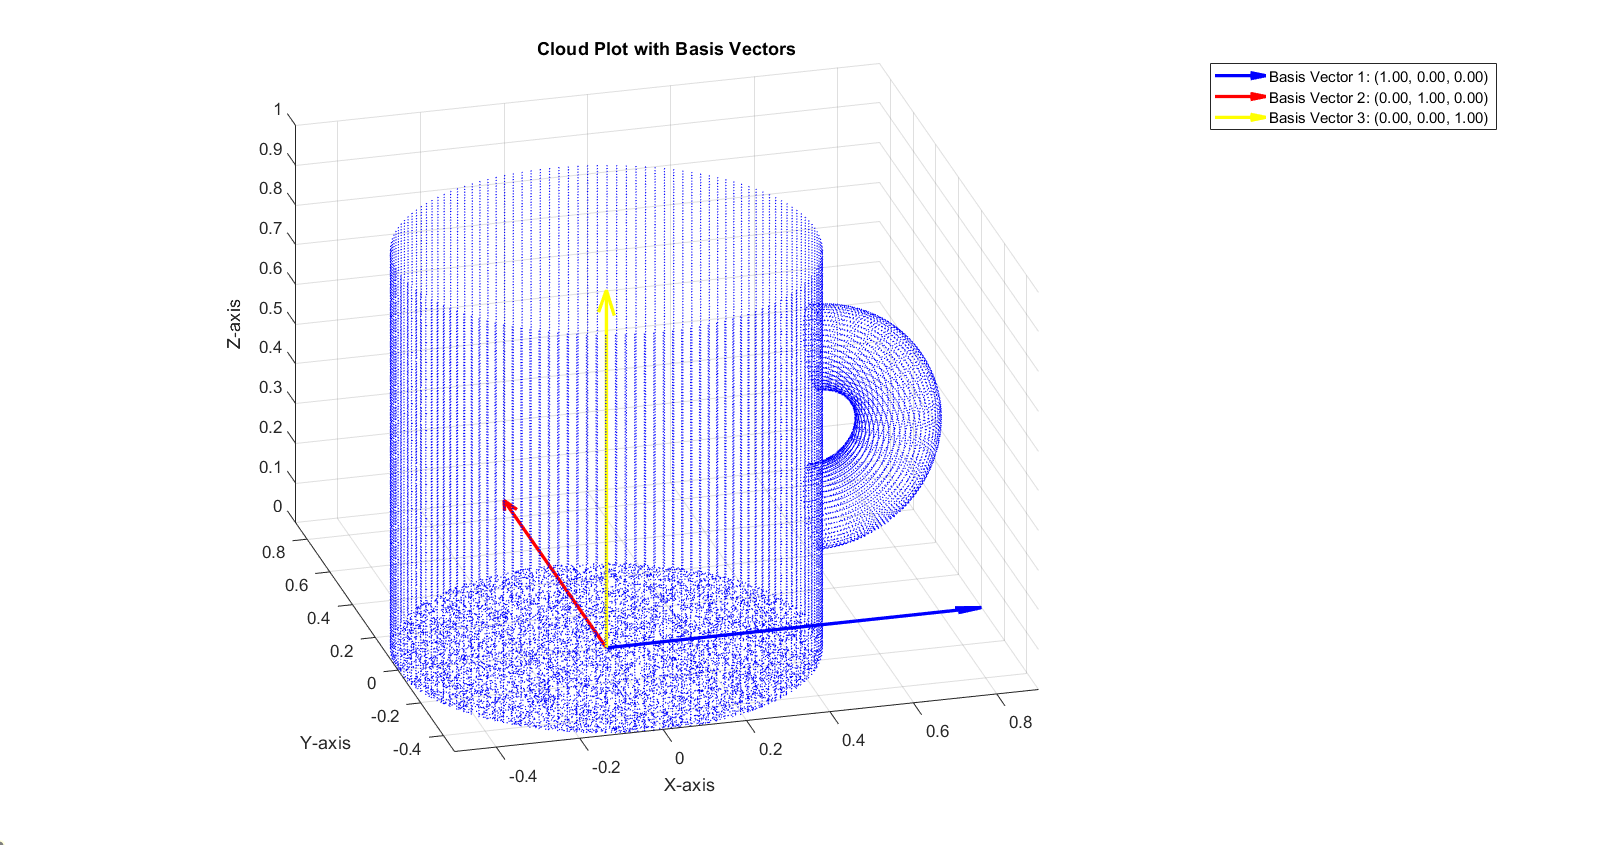
\includegraphics[width=22.22cm, height=22.22cm]{og_mug.png}
\end{center}

\begin{center}
  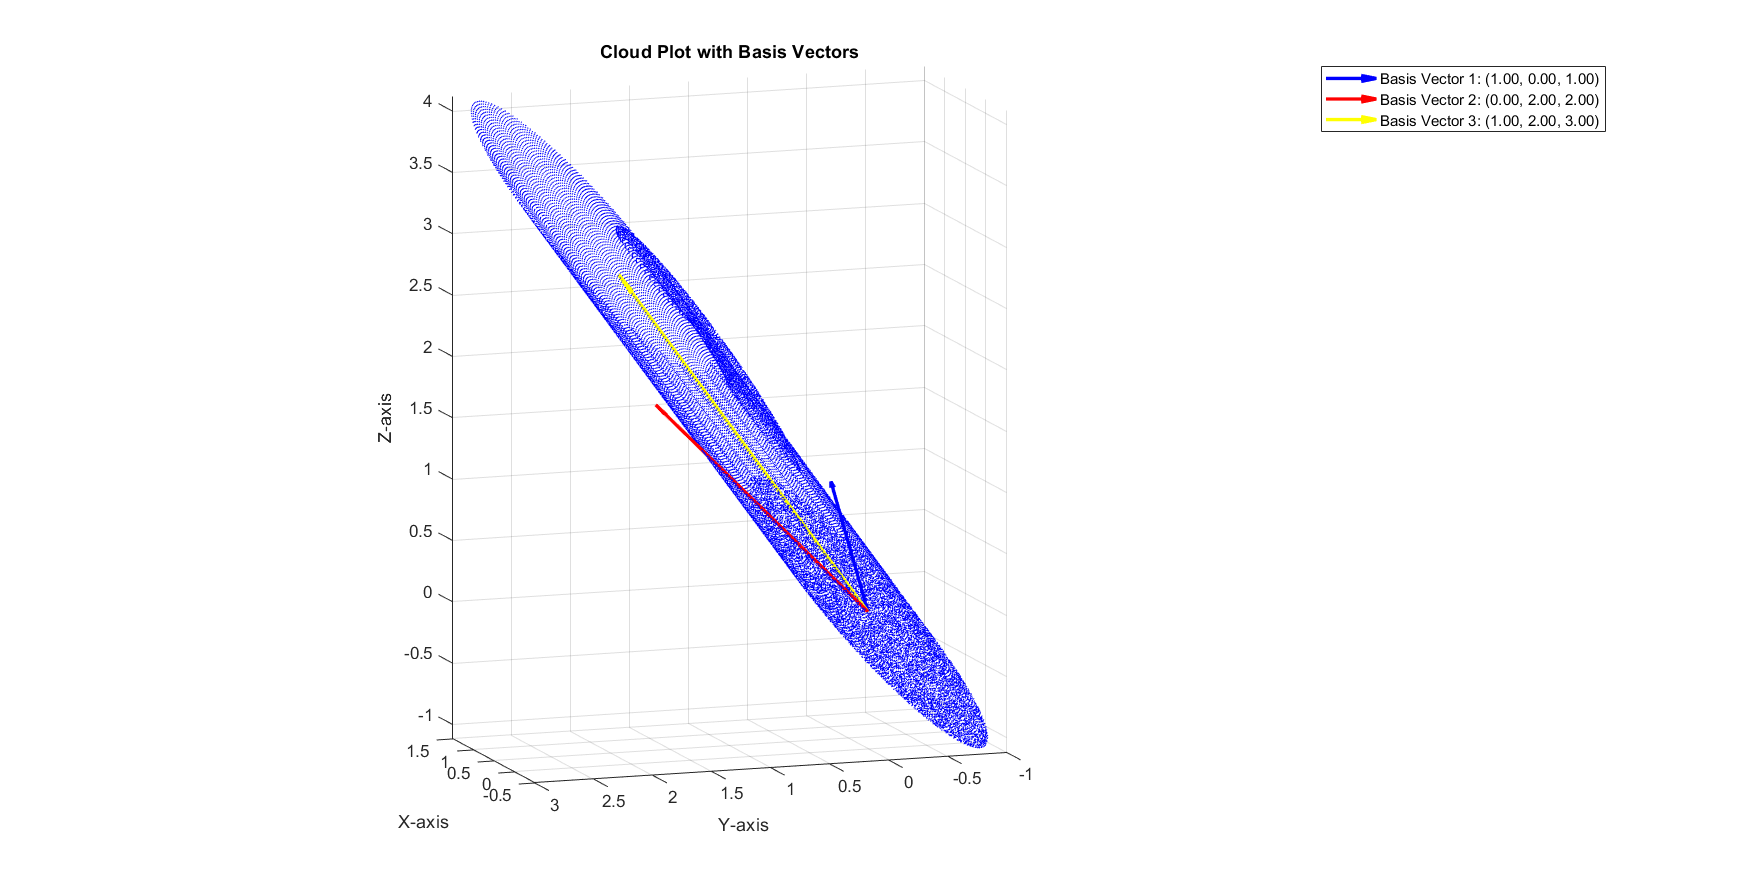
\includegraphics[width=22.22cm, height=22.22cm]{squished_mug.png}
\end{center}



Many matrices have this same effect, where the space to which vectors are sent via transformation differs from the original space of the mapping. This phenomenon is very important for the idea of invertibility (and more ideas later in the course), and deals with sets of vectors related to linear transformations called the \emph{image} and \emph{kernel} of a transformation.

First, we define the image of a transformation simply as the set of all mapped-to vectors by a transformation.

First, we discuss some terminology related to linear transformations (and more generally, functions). 

\begin{definition}
  Let $V$ and $W$ be vector spaces and $T$ a linear transformation from vectors in $V$ to vectors in $W$. That is, if $\vec{v}$ is in $V$, then $T(v)$ is in $W$.

  We call $V$ the \emph{domain} of $T$ and $W$ the \emph{codomain} of $T$.
\end{definition}

Said plainly, the domain of $T$ is the set of vectors that get mapped by $T$, and the codomain of $T$ is all of the mapped-to vectors. 

In the mug example, the set of vectors making the mug picture are in $\RR^3$, so $\RR^3$ is the domain of the transformation with matrix $A$. The resulting squished mug plane still lives in $\RR^3$, so the codomain of $T$ is still $\RR^3$. 

Since the matrix $A=\begin{bmatrix}
  1&0&0\\
  0&1&0\\
\end{bmatrix}$ is a $2x3$ matrix, it takes in vectors in $\RR^3$ and outputs vectors in $\RR^2$, so the domain is $\RR^3$ and the codomain is $\RR^2$.

This distinction could still be more refined, however. For instance we want better language to describe that the result of the mug-squishing matrix $A$ was not just $\RR^3$, but rather a plane within $\RR^3$. For this, we say that the squished-mug plane is the \emph{image} of the transformation.

START HERE

\begin{definition}\label{def:imageofT}
Let $V$ and $W$ be vector spaces and let $T:V\rightarrow W$ be a linear transformation.  

The \dfn{image} of $T$, denoted by $\mbox{im}(T)$, is the set
$$\mbox{im}(T)=\{T(\vec{v})\text{ in }W\text{ such that }\vec{v}\in V\}$$.
In other words, the image of $T$ consists of all vectors $T(\vec{v})$ that live in the target space $W$.
\end{definition}
 
\begin{example}\label{ex:image1}
Consider the linear transformation $T:\RR^3\rightarrow \RR^2$ with standard matrix
$$A=\begin{bmatrix}1&2&3\\2&4&6\end{bmatrix}$$
 
\begin{enumerate}
\item\label{item:impart1}
Find $\mbox{im}(T)$.
\item\label{item:impart2}
Illustrate the action of $T$ with a sketch.
 
\end{enumerate}
\begin{explanation}
 
\ref{item:impart1} Let $\vec{v}=\begin{bmatrix}a\\b\\c\end{bmatrix}$ then
 
$$T(\vec{v})=A\vec{v}=\begin{bmatrix}1&2&3\\2&4&6\end{bmatrix}\begin{bmatrix}a\\b\\c\end{bmatrix}=a\begin{bmatrix}1\\2\end{bmatrix}+b\begin{bmatrix}2\\4\end{bmatrix}+c\begin{bmatrix}3\\6\end{bmatrix}$$
 
Thus, every element of the image can be written as a linear combination of the columns of $A$.  We conclude that
$$\mbox{im}(T)=\mbox{span}\left(\begin{bmatrix}1\\2\end{bmatrix}, \begin{bmatrix}2\\4\end{bmatrix}, \begin{bmatrix}3\\6\end{bmatrix}\right)=\mbox{col}(A)$$
 
Every column of $A$ is a scalar multiple of $\begin{bmatrix}1\\2\end{bmatrix}$.  Thus,
 
$$\mbox{im}(T)=\mbox{span}\left(\begin{bmatrix}1\\2\end{bmatrix}, \begin{bmatrix}2\\4\end{bmatrix}, \begin{bmatrix}3\\6\end{bmatrix}\right)=\mbox{span}\left(\begin{bmatrix}1\\2\end{bmatrix}\right)$$
 
The image of $T$ is a line in $\RR^2$ determined by the vector $\begin{bmatrix}1\\2\end{bmatrix}$.
 
\ref{item:impart2} The action of $T$ can be illustrated with a sketch.
 
\begin{center}
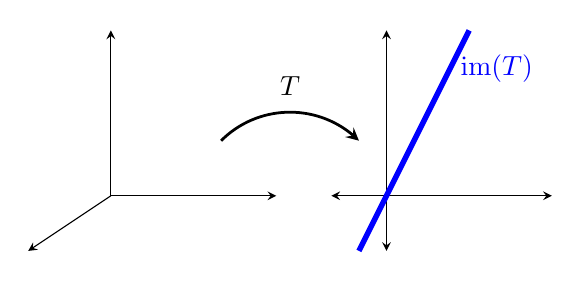
\begin{tikzpicture}[scale=.7]
 
  \draw[->] (0,0)--(3,0);
  \draw[->] (0,0)--(0,3);
  \draw[->] (0,0)--(-1.5,-1);
 
   
  \draw[<->] (4,0)--(8,0);
  \draw[<->] (5,-1)--(5,3);
  \draw[line width=2pt,blue](4.5,-1)--(6.5,3);
  \node[] at (3.25, 2)   (b) {$T$};
  \draw [->,line width=1pt,-stealth]  (2,1) to[out=45] (4.5, 1);
 \node[blue] at (7, 2.3)   (b) {$\mbox{im}(T)$};
 
\end{tikzpicture}
\end{center}
\end{explanation}
\end{example}
 
 
In Example \ref{ex:image1} we observed that the image of the linear transformation was equal to the column space of its standard matrix.  In general, it is easy to see that if $T:\RR^n\rightarrow \RR^m$ is a linear transformation with standard matrix $A$ then the following relationship holds:
$$\mbox{im}(T)=\mbox{col}(A)$$
In addition, by Theorem \ref{th:dimroweqdimcoleqrank}, we know that
$$\mbox{dim}(\mbox{im}(T))=\mbox{dim}(\mbox{col}(A))=\mbox{rank}(A)$$
 
 
 
\begin{example}\label{ex:image2}
Let $T:\RR^5\rightarrow \RR^4$ be a linear transformation with standard matrix $$A=\begin{bmatrix}1 & 2 & 2 &-1 & 0\\-1 & 3 & 1 & 0 & -1\\3 & 0 & 0 & 3 & 6\\ 1 & -1 & 1 & -2 & -1\end{bmatrix}$$
Find $\mbox{im}(T)$ and $\mbox{dim}(\mbox{im}(T))$.
\begin{explanation}
As in Example \ref{ex:image1}, the image of $T$ is given by
$$\mbox{im}(T)=\mbox{span}\left(\begin{bmatrix}1\\-1\\3\\1\end{bmatrix}, \begin{bmatrix}2\\3\\0\\-1\end{bmatrix}, \begin{bmatrix}2\\1\\0\\1\end{bmatrix}, \begin{bmatrix}-1\\0\\3\\-2\end{bmatrix}, \begin{bmatrix}0\\-1\\6\\-1\end{bmatrix}\right)=\mbox{col}(A)$$
This time it is harder to detect the vectors that can be eliminated from the spanning set without affecting the span.  We have to rely on the reduced row-echelon form of $A$.
 
$$\begin{bmatrix}1 & 2 & 2 &-1 & 0\\-1 & 3 & 1 & 0 & -1\\3 & 0 & 0 & 3 & 6\\ 1 & -1 & 1 & -2 & -1\end{bmatrix}  \rightsquigarrow \begin{bmatrix} 1 & 0 & 0 & 1 & 2\\0 & 1 & 0 & 1 & 1\\0 & 0 & 1 & -2 & -2\\ 0 & 0 & 0 & 0 & 0 \end{bmatrix}$$
 
We can see that $\mbox{rank}(A)=3$, so $\mbox{dim}(\mbox{im}(T))=3$. 
 
To identify vectors that span $\mbox{im}(T)$, we turn to Procedure \ref{proc:colspace}.  We identify the first three columns as pivot columns.  These columns are linearly independent and span $\mbox{col}(A)$.  Therefore,
$$\mbox{im}(T)=\mbox{col}(A)=\mbox{span}\left(\begin{bmatrix}1\\-1\\3\\1\end{bmatrix}, \begin{bmatrix}2\\3\\0\\-1\end{bmatrix}, \begin{bmatrix}2\\1\\0\\1\end{bmatrix}\right)$$
\end{explanation}
\end{example}

By Theorem \ref{th:span_is_subspace} and Definition \ref{def:colspace}, we know that for an $m\times n$ matrix $A$, $\mbox{col}(A)$ is a subspace of $\RR^m$.  However, when vector spaces other than $\RR^m$ are involved, it is not yet clear that $\mbox{im}(T)$ is a subspace of the codomain. The following theorem resolves this issue.
 
\begin{theorem}\label{th:imagesubspace}
Let $T:V\rightarrow W$ be a linear transformation.  Then $\mbox{im}(T)$ is a subspace of $W$.
\end{theorem}
\begin{proof}
To show that $\mbox{im}(T)$ is a subspace, we need to show that $\mbox{im}(T)$ is closed under addition and scalar multiplication.
 
Suppose $\vec{w}_1$ and $\vec{w}_2$ are in $\mbox{im}(T)$.  Then there are vectors $\vec{v}_1$ and $\vec{v}_2$ in $V$ such that $T(\vec{v}_1)=\vec{w}_1$ and $T(\vec{v}_2)=\vec{w}_2$.  Then
$$\vec{w}_1+\vec{w}_2=T(\vec{v}_1)+T(\vec{v}_2)=T(\vec{v}_1+\vec{v}_2)$$
This shows that $\vec{w}_1+\vec{w}_2$ is in $\mbox{im}(T)$.
 
For any scalar $a$, we have:
$$a\vec{w}_1=aT(\vec{v}_1)=T(a\vec{v}_1)$$
This shows that $a\vec{w}_1$ is in $\mbox{im}(T)$.
 
\end{proof}
 
We can now define the rank of a linear transformation.
 
\begin{definition}\label{def:rankofT}
The \dfn{rank} of a linear transformation $T:V\rightarrow W$, is the dimension of the image of $T$.
$$\mbox{rank}(T)=\mbox{dim}(\mbox{im}(T))$$
\end{definition}
 
This definition gives us the following relationship between the rank of a linear transformation $T:\RR^n\rightarrow\RR^m$ and the rank of the standard matrix $A$ associated with it.
 
\begin{formula}\label{form:rankTrankA}
$$\mbox{rank}(A) = \mbox{dim}(\mbox{col}(A))=\mbox{dim}(\mbox{im}(T))=\mbox{rank}(T)$$
\end{formula}
 
%Note that since  $\mbox{rank}(A) = \mbox{dim}(\mbox{col}(A))=\mbox{dim}(\mbox{im}(T))$, our definitions of the rank of a linear transformation and the rank of its associated standard matrix are in agreement.
 
\subsection*{The Kernel of a Linear Transformation}
 
\begin{definition}\label{def:kernel}
Let $V$ and $W$ be vector spaces, and let $T:V\rightarrow W$ be a linear transformation.  The \dfn{kernel} of $T$, denoted by $\mbox{ker}(T)$, is the set
$$\mbox{ker}(T)=\{\vec{v}:T(\vec{v})=\vec{0}\}$$
In other words, the kernel of $T$ consists of all vectors of $V$ that map to $\vec{0}$ in $W$.
\end{definition}
It is important to pay attention to the locations of the kernel and the image.  We already proved that $\mbox{im}(T)$ is a subspace of the codomain.  In contrast, $\mbox{ker}(T)$ is located in the domain.  (We will prove shortly that it is a subspace of the domain.)
 
\begin{center}
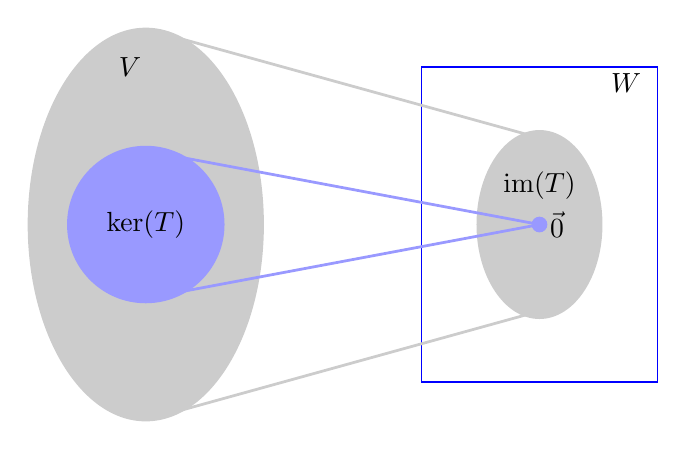
\begin{tikzpicture}
\fill[gray!40] (0,0) ellipse (1.5cm and 2.5cm);
\fill[blue!40!white] (0,0) ellipse (1cm and 1cm)node[black]{$\mbox{ker}(T)$};
 
\draw[blue] (3.5,2) rectangle (6.5,-2);
\node[] at (6.1, 1.8)   (b) {$W$};
\fill[gray!40] (5,0) ellipse (0.8cm and 1.2cm);
\fill[blue!40!white] (5,0) circle (0.1cm);
 
\draw[gray!40,line width=1pt](0.3,2.4)--(5,1.1);
\node[] at (-0.2, 2)   (b) {$V$};
\node[] at (5, 0.5)   (b) {$\mbox{im}(T)$};
\draw[gray!40, line width=1pt](0.3,-2.4)--(5,-1.1);
 
\draw[blue!40!white, line width=1pt](0.2,.9)--(5,0);
\draw[blue!40!white, line width=1pt](0.2,-0.9)--(5,0)node[below, right][black]{$\vec{0}$};
 
\end{tikzpicture}
\end{center}
 
 
\begin{example}\label{ex:kernel} Let $T:\RR^5\rightarrow \RR^4$ be a linear transformation with standard matrix $$A=\begin{bmatrix}1 & 2 & 2 &-1 & 0\\-1 & 3 & 1 & 0 & -1\\3 & 0 & 0 & 3 & 6\\ 1 & -1 & 1 & -2 & -1\end{bmatrix}$$
\begin{enumerate}
\item \label{item:kernelT}
Find $\mbox{ker}(T)$
\item \label{item:dimkernelT}
Is $\mbox{ker}(T)$ a subspace of $\RR^5$?  If so, find $\mbox{dim}(\mbox{ker}(T))$.
\end{enumerate}
\begin{explanation}
\ref{item:kernelT} To find the kernel of $T$, we need to find all vectors of $\RR^5$ that map to $\vec{0}$ in $\RR^4$.  This amounts to solving the equation $A\vec{x}=\vec{0}$.
 
Gauss-Jordan elimination yields:
 
$$\begin{bmatrix}1 & 2 & 2 &-1 & 0\\-1 & 3 & 1 & 0 & -1\\3 & 0 & 0 & 3 & 6\\ 1 & -1 & 1 & -2 & -1\end{bmatrix}  \rightsquigarrow \begin{bmatrix} 1 & 0 & 0 & 1 & 2\\0 & 1 & 0 & 1 & 1\\0 & 0 & 1 & -2 & -2\\ 0 & 0 & 0 & 0 & 0 \end{bmatrix}$$
 
Thus, the kernel of $T$ consists of all elements of the form:
$$\begin{bmatrix}-1\\-1\\2\\1\\0\end{bmatrix}s+\begin{bmatrix}-2\\-1\\2\\0\\1\end{bmatrix}t$$
 
We conclude that
$$\mbox{ker}(T)=\mbox{span}\left(\begin{bmatrix}-1\\-1\\2\\1\\0\end{bmatrix}, \begin{bmatrix}-2\\-1\\2\\0\\1\end{bmatrix}\right)$$
 
\ref{item:dimkernelT}  Since $\mbox{ker}(T)$ is the span of two vectors of $\RR^5$, we know that $\mbox{ker}(T)$ is a subspace of $\RR^5$. (See Theorem \ref{th:span_is_subspace}.)  Observe that the two vectors in the spanning set are linearly independent. (How can we see this without performing computations?)  Therefore $\mbox{dim}(\mbox{ker}(T))=2$.
\end{explanation}
\end{example}
 
 
Recall that the \dfn{null space} of a matrix $A$ is defined to be set of all solutions to the homogeneous equation $A\vec{x}=\vec{0}$. This means that  if $T:\RR^n\rightarrow \RR^m$ is a linear transformation with standard matrix $A$ then
$$\mbox{ker}(T)=\mbox{null}(A)$$
 
We know that $\mbox{null}(A)$ of an $m\times n$ matrix is a subspace of $\RR^n$. (See Theorem \ref{th:nullsubspacern}.)  We conclude this section by showing that even when vector spaces other than $\RR^n$ are involved, the kernel of a linear transformation is a subspace of the domain of the transformation.
\begin{theorem}\label{th:kersubspace} Let $T:V\rightarrow W$ be a linear transformation, then $\mbox{ker}(T)$ is a subspace of $V$.
\end{theorem}
\begin{proof}
To show that $\mbox{ker}(T)$ is a subspace, we need to show that $\mbox{ker}(T)$ is closed under addition and scalar multiplication.
 
Suppose that $\vec{v}_1$ and $\vec{v}_2$ are in $\mbox{ker}(T)$.  Then,
$$T(\vec{v}_1+\vec{v}_2)=T(\vec{v}_1)+T(\vec{v}_2)=\vec{0}+\vec{0}=\vec{0}$$
This shows that $\vec{v}_1+\vec{v}_2$ is in $\mbox{ker}(T)$.
 
For any scalar $a$ we have:
$$T(a\vec{v}_1)=aT(\vec{v}_1)=a\vec{0}=\vec{0}$$
This shows that $a\vec{v}_1$ is in $\mbox{ker}(T)$.
 
\end{proof}
 
 
 
\begin{definition}\label{def:nullityT}
The \dfn{nullity} of a linear transformation $T:V\rightarrow W$, is the dimension of the kernel of $T$.
$$\mbox{nullity}(T)=\mbox{dim}(\mbox{ker}(T))$$
\end{definition}
 
This definition gives us the following relationship between nullity of a linear transformation $T:\RR^n\rightarrow\RR^m$ and the nullity of the standard matrix $A$ associated with it.
 
\begin{formula}\label{form:nullTnullA}
$$\mbox{nullity}(A) = \mbox{dim}(\mbox{null}(A))=\mbox{dim}(\mbox{ker}(T))=\mbox{nullity}(T)$$
\end{formula}
 
 
%Notice that since the nullity of a matrix $A$ was defined as $\mbox{nullity}(A) = \mbox{dim}(\mbox{null}(A))$ (Definition \ref{def:matrixnullity} of VSP-0040), and the kernel of a linear transformation $T:\RR^n\rightarrow \RR^m$ is the null space of its associated standard matrix, our definitions of nullity are in agreement.
 
\subsection*{Rank-Nullity Theorem for Linear Transformations}
 
In Examples \ref{ex:image2} and \ref{ex:kernel}, we found the image and the kernel of the linear transformation $T:\RR^5\rightarrow \RR^4$ with standard matrix
 
$$A=\begin{bmatrix}1 & 2 & 2 &-1 & 0\\-1 & 3 & 1 & 0 & -1\\3 & 0 & 0 & 3 & 6\\ 1 & -1 & 1 & -2 & -1\end{bmatrix}$$
 
We also found that
$$\mbox{rank}(T)=\mbox{dim}(\mbox{im}(T))=\mbox{dim}(\mbox{col}(A))=\mbox{rank}(A)=3$$
and
$$\mbox{nullity}(T)=\mbox{dim}(\mbox{ker}(T))=\mbox{dim}(\mbox{null}(A))=\mbox{nullity}(A)=2$$
 
Because of Rank-Nullity Theorem for matrices (Theorem \ref{th:matrixranknullity}), it is not surprising that
$$\mbox{rank}(T)+\mbox{nullity}(T)=3+2=5=\mbox{dim}(\RR^5)$$
 
 
The following theorem is a generalization of this result.
 
\begin{theorem}\label{th:ranknullityforT}
Let $T:V\rightarrow W$ be a linear transformation.  Suppose $\mbox{dim}(V)=n$, then
$$\mbox{rank}(T)+\mbox{nullity}(T)=n$$
\end{theorem}
 
\begin{proof}
By Theorem \ref{th:imagesubspace}, $\mbox{im}(T)$ is a subspace of $W$.  There exists a basis for $\mbox{im}(T)$ of the form $\{T(\vec{v}_1), \ldots,T(\vec{v}_r)\}$.  By Theorem \ref{th:kersubspace}, $\mbox{ker}(T)$ is a subspace of $V$.  Let $\{\vec{u}_1,\ldots,\vec{u}_s\}$ be a basis for $\mbox{ker}(T)$.
 
We will show that $\{\vec{u}_1,\ldots ,\vec{u}_s, \vec{v}_1,\ldots ,\vec{v}_r\}$ is a basis for $V$.
 
For any vector $\vec{v}$ in $V$, we have:
$$T(\vec{v})=c_1T(\vec{v}_1)+\ldots +c_rT(\vec{v}_r)$$
for some scalars $c_i$ $(1\leq i\leq r)$.
Thus,
$$T(\vec{v})-\big(c_1T(\vec{v}_1)+\ldots +c_rT(\vec{v}_r)\big)=\vec{0}$$
By linearity,
$$T((\vec{v}-(c_1\vec{v}_1+\ldots +c_r\vec{v}_r))=\vec{0}$$
Therefore $\vec{v}-(c_1\vec{v}_1+\ldots +c_r\vec{v}_r)$ is in $\mbox{ker}(T)$.
 
Hence there are scalars $a_i$ $(1\leq i\leq s)$ such that
$$\vec{v}-(c_1\vec{v}_1+\ldots +c_r\vec{v}_r)=a_1\vec{u}_1+\ldots +a_s\vec{u}_s$$
Thus,
$$\vec{v}=(c_1\vec{v}_1+\ldots +c_r\vec{v}_r)+(a_1\vec{u}_1+\ldots +a_s\vec{u}_s)$$
 
We conclude that
$$V=\mbox{span}(\vec{u}_1,\ldots ,\vec{u}_s, \vec{v}_1,\ldots ,\vec{v}_r)$$
 
Now we need to show that $\{\vec{u}_1,\ldots ,\vec{u}_s, \vec{v}_1,\ldots ,\vec{v}_r\}$ is linearly independent.
 
Suppose
\begin{align}\label{eq:kerplusimproof} c_1\vec{v}_1+\ldots +c_r\vec{v}_r+a_1\vec{u}_1+\ldots +a_s\vec{u}_s=\vec{0}\end{align}
Applying $T$ to both sides, we get
$$T(c_1\vec{v}_1+\ldots +c_r\vec{v}_r+a_1\vec{u}_1+\ldots +a_s\vec{u}_s)=T(\vec{0})$$
$$c_1T(\vec{v}_1)+\ldots +c_rT(\vec{v}_r)+a_1T(\vec{u}_1)+\ldots +a_sT(\vec{u}_s)=\vec{0}$$
 
But $T(\vec{u}_i)=\vec{0}$ for $1\leq i\leq s$, thus
$$c_1T(\vec{v}_1)+\ldots +c_rT(\vec{v}_r)=\vec{0}$$
Since $\{T(\vec{v}_1),\ldots ,T(\vec{v}_r)\}$ is linearly independent, it follows that each $c_i=0$. 
 
But then Equation (\ref{eq:kerplusimproof}) implies that $a_1\vec{u}_1+\ldots +a_s\vec{u}_s=\vec{0}$.  Because $\{\vec{u}_1, \ldots ,\vec{u}_s\}$ is linearly independent, it follows that each $a_i=0$. 
 
We conclude that $\{\vec{u}_1,\ldots ,\vec{u}_s,\vec{v}_1,\ldots ,\vec{v}_r\}$ is a basis for $V$.  Thus,
 
$$\mbox{dim}(\mbox{ker}(T))+\mbox{dim}(\mbox{im}(T))=s+r=n$$
\end{proof}
 
\section*{Practice Problems}
\begin{problem}
Describe the image and find the rank for each linear transformation $T:\RR^n\rightarrow \RR^m$ with standard matrix $A$ given below.
  \begin{problem}\label{prob:imagerankoflintrans1}
  $T:\RR^5\rightarrow \RR^2$, $A=\begin{bmatrix}3&2&4&7&1\\-1&-9&7&6&8\end{bmatrix}$.
   
  \begin{multipleChoice}
  \choice[correct]{$\mbox{im}(T)=\RR^2$}
  \choice{$\mbox{im}(T)$ is a line in $\RR^2$}
  \choice{$\mbox{im}(T)=\{\vec{0}\}$ }
  \choice{$\mbox{im}(T)=\RR^5$}
  \choice{$\mbox{im}(T)$ is a plane in $\RR^5$}
\end{multipleChoice}
   
  $\mbox{rank}(T)=\answer{2}$
  \end{problem}
   
  \begin{problem}\label{prob:imagerankoflintrans2}
  $T:\RR^2\rightarrow\RR^3$, $A=\begin{bmatrix}1&1\\1&1\\1&1\end{bmatrix}$
   
  \begin{multipleChoice}
  \choice{$\mbox{im}(T)=\RR^3$}
  \choice{$\mbox{im}(T)$ is a line in $\RR^2$}
  \choice[correct]{$\mbox{im}(T)$ is a line in $\RR^3$}
  \choice{$\mbox{im}(T)=\{\vec{0}\}$ }
  \choice{$\mbox{im}(T)$ is a plane in $\RR^3$}
\end{multipleChoice}
   
  $\mbox{rank}(T)=\answer{1}$
  \end{problem}
\end{problem}
 
 
\begin{problem}\label{prob:sametrans} Suppose linear transformations $T:\RR^2\rightarrow \RR^2$ and $S:\RR^2\rightarrow \RR^2$ are such that  $\mbox{im}(T)=\mbox{im}(S)=\mbox{span}\left(\begin{bmatrix}1\\-3\end{bmatrix}\right)$.  Does this mean that $T$ and $S$ are the same transformation?  Justify your claim.
\end{problem}
 
\begin{problem}
Describe the kernel and find the nullity for each linear transformation $T:\RR^n\rightarrow \RR^m$ with standard matrix $A$ given below.
 
\begin{problem}\label{prob:kerandnullityT1}
$T:\RR^3\rightarrow \RR^2$, $A=\begin{bmatrix}2&1&0\\-1&1&-3\end{bmatrix}$.
 
\begin{multipleChoice}
  \choice{$\mbox{ker}(T)=\RR^3$}
  \choice{$\mbox{ker}(T)=\{\vec{0}\}$ }
  \choice{$\mbox{ker}(T)=\RR^2$}
  \choice{$\mbox{ker}(T)$ is a plane in $\RR^3$}
   \choice[correct]{$\mbox{ker}(T)$ is a line in $\RR^3$}
\end{multipleChoice}
 
$\mbox{nullity}(T)=\answer{1}$
\end{problem}
 
\begin{problem}\label{prob:kerandnullityT2}
$T:\RR^2\rightarrow \RR^2$, $A=\begin{bmatrix}2&-1\\3&0\end{bmatrix}$.
 
\begin{multipleChoice}
  \choice{$\mbox{ker}(T)=\RR^2$}
  \choice[correct]{$\mbox{ker}(T)=\{\vec{0}\}$ }
   \choice{$\mbox{ker}(T)$ is a line in $\RR^2$}
\end{multipleChoice}
 
$\mbox{nullity}(T)=\answer{0}$
\end{problem}
 
\begin{problem}\label{prob:kerandnullityT3}
$T:\RR^3\rightarrow \RR^5$, $A=\begin{bmatrix}1&2&-1\\1&2&-1\\1&2&-1\\1&2&-1\\1&2&-1\end{bmatrix}$
 
\begin{multipleChoice}
 \choice[correct]{$\mbox{ker}(T)$ is a plane in $\RR^3$}
 \choice{$\mbox{ker}(T)$ is a line in $\RR^3$}
     \choice{$\mbox{ker}(T)$ is a line in $\RR^5$}
 \choice{$\mbox{ker}(T)=\RR^3$}
  \choice{$\mbox{ker}(T)=\{\vec{0}\}$ }
   
\end{multipleChoice}
 
$\mbox{nullity}(T)=\answer{2}$
\end{problem}
\end{problem}
 
\begin{problem}\label{prob:ranknullityT4}
Suppose a linear transformation $T:\RR^3\rightarrow \RR^3$ is such that $\mbox{im}(T)$ is a plane in $\RR^3$.  Then
$$\mbox{rank}(T)=\answer{2}$$ $$\mbox{nullity}(T)=\answer{1}$$
\end{problem}
 
\begin{problem}\label{prob:ranknullityT5}
Suppose a linear transformation $T:\RR^5\rightarrow \RR^5$ is such that $T(\vec{v})=\vec{0}$ for all $\vec{v}$ in $\RR^5$.  Then
$$\mbox{rank}(T)=\answer{0}$$ $$\mbox{nullity}(T)=\answer{5}$$
\end{problem}
 
\begin{problem}\label{prob:findimkergivenrref} Let $T:\RR^6\rightarrow \RR^4$ be a linear transformation with standard matrix
$$A=\begin{bmatrix}2&-1&1&-2&1&1\\1&2&3&6&-4&1\\0&2&2&4&-2&-1\\1&3&2&6&-3&2\end{bmatrix}$$
Find $\mbox{im}(T)$ and $\mbox{ker}(T)$ if the reduced row-echelon form of $A$ is
$$\text{rref}(A)=\begin{bmatrix}1&0&0&1&-1&0\\0&1&0&1&0&0\\0&0&1&1&-1&0\\0&0&0&0&0&1\end{bmatrix}$$
\end{problem}
\begin{problem}\label{prob:findimageandkernellintrans} Let $V=\mbox{span}\left(\begin{bmatrix}1\\1\end{bmatrix}\right)$, and let $T:V\rightarrow \RR^2$ be a linear transformation defined by
$T(\vec{v})=2\vec{v}$.  Find $\mbox{im}(T)$ and $\mbox{ker}(T)$.
\end{problem}
 
\begin{problem}\label{prob:ranknullitytrans}
Suppose a linear transformation $T$ is induced by a $4\times 6$ matrix $A$.  Let $S$ be a linear transformation induced by $A^T$.  Find $\mbox{nullity}(S)$, if $\mbox{nullity}(T)=3$.  Prove your claim.
\end{problem}
 
 

\end{document}